\chapter{Grundlagen}
\label{chap:grundlagen}
Das Kapitel Grundlagen behandelt die Themen, die in mehreren Abschnitten dieser Arbeit relevant sind. Dabei handelt es sich um das Robot Operation System, die verwendeten Koordinatensysteme und die Transformation zwischen ihnen.

\section{Das Robot Operation System \gls{ros}}
\label{sec:ros}
Ziel dieses Unterkapitel ist es das Betriebssystem \gls{ros} vorzustellen. Wie es aufgebaut ist und welche Vorz�ge es besitzt.\\

\gls{ros} stellt dem Softwareentwickler Bibliotheken und Werkzeuge zur Verf�gung, die Helfen Roboteranwendungen zu erstellen. Das auf einem \gls{ip}-basierende  modularen Kommunikationsframework erm�glicht die Verkn�pfung von Anwendungssoftware, Sensoren und Aktoren sogar unter mehreren Robotern. Die Grundlage daf�r ist die sogenannte Hardwareabstraktion. Dabei wird durch hardwarespezifische Module erreicht, das Komponenten unterschiedlicher Hersteller miteinander verbunden werden k�nnen. In unserem Fall Hokuyo Lasersanner und \gls{asctec} \gls{fcu}. Au�erdem erm�glicht es eine hardwareunabh�ngige Programmierung. Diese kann in den Programmiersprachen C/C++ oder in Python erfolgen.Jede Hardwareabstraktion oder Anwendung wird als Node, bzw. Konten bezeichnet und l�uft als eigener Prozess.
\begin{figure}
	\centering
	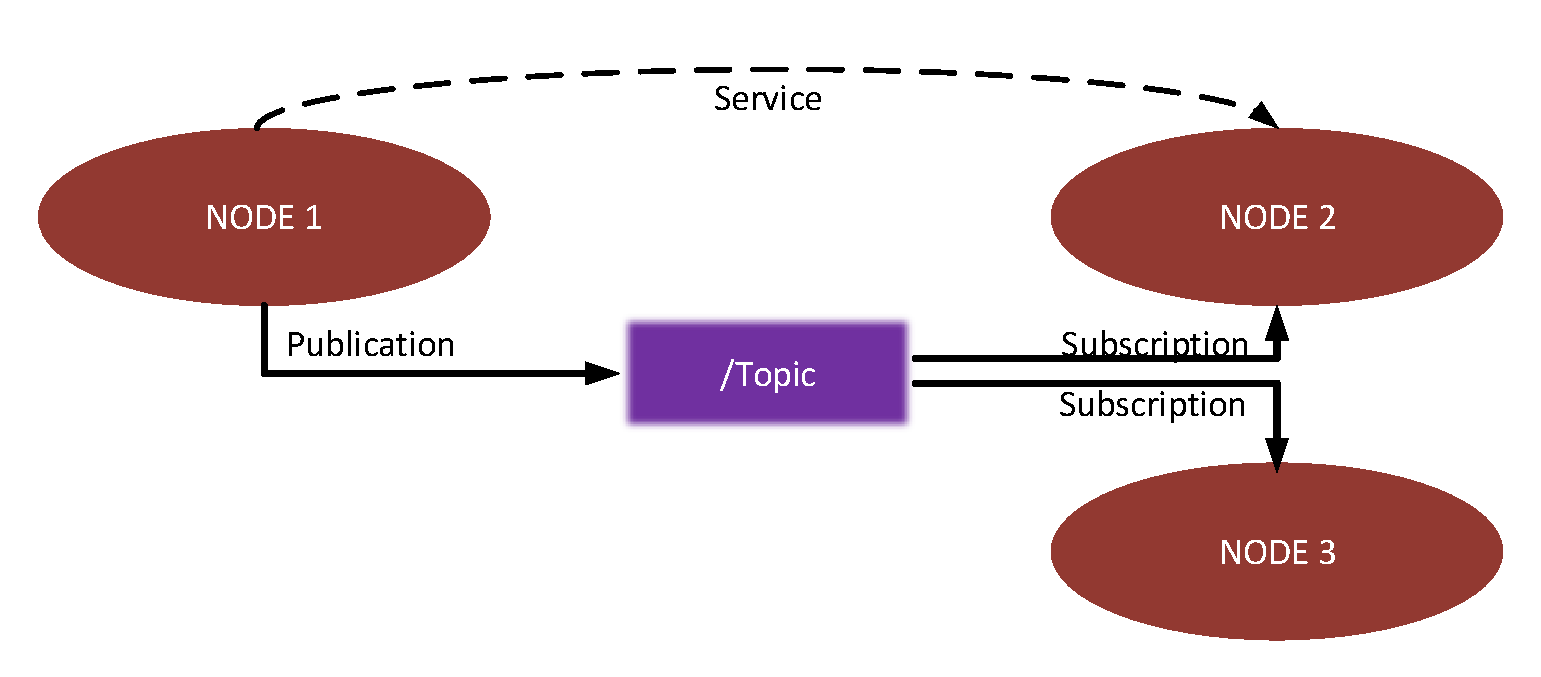
\includegraphics[width = 0.75\textwidth]{images/TopicUndService}
	\caption[Node Kommunikation]{Kommunikation von Node1 zu Node2 �ber ein Topic sowie einem Service}
	\label{fig:node_kommunikation}
\end{figure}


Der Austausch von Daten zwischen den Nodes erfolgt �ber so genannte Topics (Abbildung \ref{fig:node_kommunikation}]. Dabei werden von den Knoten Nachrichten (engl. Messages) in Topics gepostet und somit ver�ffentlicht (publication). Ben�tigt ein weiter Knoten den Inhalt dieses Topic kann er dieses abonnieren (subscription). Sobald die Nachricht im Knoten aktualisiert wurde, wird sie dem abonnierenden Knoten �bertragen. Dabei sind Knoten nicht auf ein Topic beschr�nkt. Es k�nnen beliebig viele Topics beschrieben oder empfangen werden. Alternative dieser Art der asynchronen Daten�bertragung, biete eine Synchrone Kommunikation zwischen zwei Nodes �ber Services. Dabei wird auf einem Knoten ein Service gestartet. Dieser dient nun als Server und agiert nach dem Anfrage-Antwort-Prinzip. Schickt nun ein anderer Knoten eine Anfrage, wird im die Nachricht zu gesendet.

\begin{figure}
	\centering
	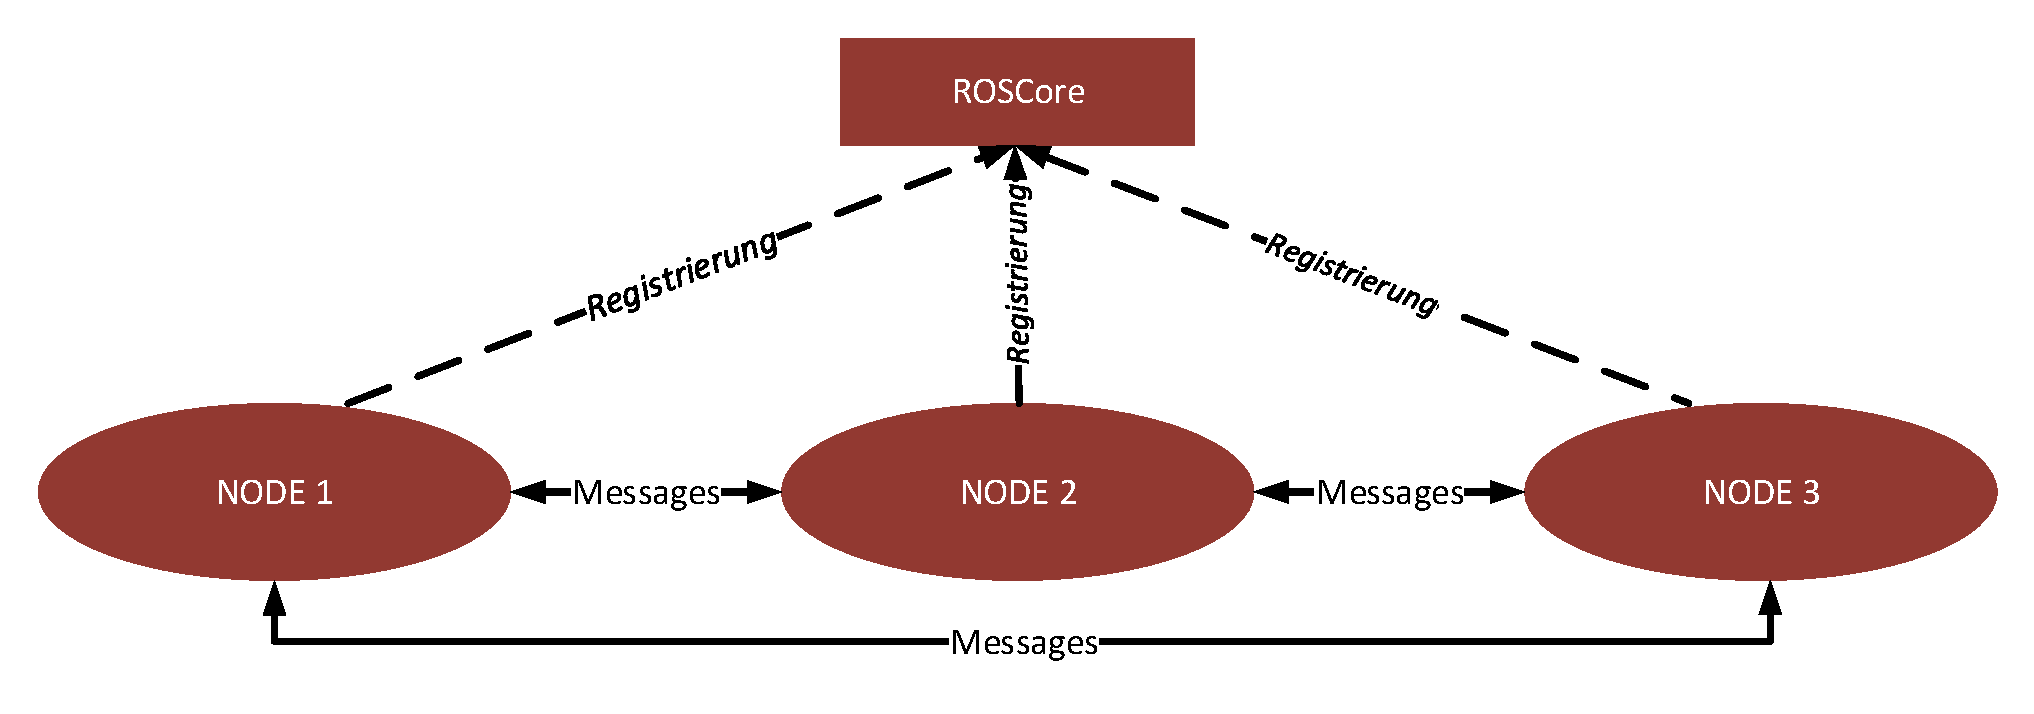
\includegraphics[width = \textwidth]{images/MasterAndNode}
	\caption[Registrierung der Knoten]{Registrierung der Knoten}
	\label{fig:node_master}
\end{figure}

Die Verwaltung aller Nodes, Topics sowie Services erfolgt �ber einen Master dem ROSCore (Abbildung\ref{fig:node_master}).  Hier melden sich alle Knoten an. Durch die zentrale Registrierung k�nnen  Nodes sich gegenseitig finden. Sobald sie sich gefunden haben, kommunizieren diese direkt miteinander.

